% -------------------------------------------------------------------
% Masterarbeit
% Kapitel 4: Implementierungstechniken
% Autor: Daniel Fritz
% Datum: 09.04.2016
% -------------------------------------------------------------------

\chapter{Implementierungstechniken}\label{chp:4:implementierungstechniken}
Dieses Kapitel stellt dar, aus welchen Teilen die Implementierung der Sprache aufgebaut ist. Ihre Funktion, ihre Implementierung und mögliche Alternativen werden gezeigt. Aufgrund des Inhalts dieser Arbeit beschränken sich Beispiele und Beschreibungen auch auf Java. Die Konzepte können jedoch auch auf andere Programmiersprachen übertragen werden. In den Abschnitten \ref{sct:4.1:eigenschaften} und \ref{sct:4.2:datenstrukturen} werden allgemeine Techniken vorgestellt, die oft bei der Implementierung einer Programmiersprache, insbesondere einer internen DSL verwendet werden. Die restlichen Abschnitte dieses Kapitels widmen sich der Implementierungen im Rahmen dieser Abschlussarbeit.

\section{Eigenschaften der Sprache}\label{sct:4.1:eigenschaften}
Der Bezug auf ein bestimmtes Arbeitsgebiet ist für eine Domänenspezifische Sprache obligatorisch. Es gibt noch weitere Eigenschaften\todo{anderes Wort?}, die häufig mit internen DSLs in Verbindung gebracht werden, auch wenn sie nicht zwingend erforderlich sind. Jedoch steigern sie die Lesbarkeit der Sprache und die Produktivität bei der Arbeit mit ihr. An dieser Stelle sollen diese Eigenschaften kurz beschrieben werden und beispielhaft \todo{richtiges Wort?} erklärt werden, wie man sie erreicht.

\subsection{Method Chaining}\label{ssct:4.1.1:chaining}
Method Chaining, das Aneinanderreihen von Methoden, wird von vielen direkt mit dem Aussehen einer internen DSL verbunden. Es ist zwar nicht zwingend notwendig, Method Chaining in einer internen DSL zu verwenden, jedoch ist es eine sehr nützliche Technik mit der man den Sprachfluss und die Lesbarkeit einer Sprache deutlich verbessern kann\cite{book:fowlerDSL}. Ein kurzes Beispiel soll dies verdeutlichen.

Dafür nehmen wir an, dass eine Klasse \emph{Rezept} alle Zutaten für ein bestimmtes Rezept hält. Da eine Vielzahl an Zutaten möglich ist, aber immer nur ein paar wenige für ein einzelnes Rezept nötig sind, werden sie der Klasse nicht per Konstruktor sondern per set-Methode übergeben. Normalerweise würde das folgendermaßen aussehen (alle Code-Beispiele sind in Java):\\

\begin{lstlisting}[caption=Erstellung eines Rezepts auf normale Weise]
	Recipe cake = new Recipe();
	cake.setButter(200);
	cake.setSugar(300);
	cake.setEggs(4);
	cake.setMilk(200);
	cake.setFlour(500);
\end{lstlisting}

\noindent
Dasselbe Rezept würde man mithilfe von Method Chaining auf die folgende Weise zusammenstellen:\\


\begin{lstlisting}[caption=Erstellung desselben Rezepts mit Method Chaining]
	Recipe cake = new Recipe();
	cake.butter(200).sugar(300).eggs(4).milk(200).flour(500);
\end{lstlisting}

Um dieses Verhalten zu erreichen, müssen die einzelnen setter-Methoden anders als gewohnt implementiert werden. Üblicherweise würde eine Methode der Klasse so aussehen:\\

\begin{lstlisting}[caption={set-Methode, implementiert zur Aneinaderreihung}]
	public Recipe butter(int butterInGrams) {
		this.butter = butterInGrams;
	}
\end{lstlisting}

Um sie verketten zu können, müsste man dieselbe Methode folgendermaßen implementieren:\\

\begin{lstlisting}[caption=set-Methode in der üblichen Implementierung]
	public void setButter(int butterInGrams) {
		this.butter = butterInGrams;
	}
\end{lstlisting}

\subsection{Method Nesting}\label{ssct:4.1.2:nesting}
Method Nesting beschreibt das Verschachteln von Funktionen um hierarchische Strukturen abzubilden, insbesondere rekursive Aufrufe\cite{book:fowlerDSL}, \cite{vl:drachen:teil3}. Dies wird erreicht, indem Rückgabewerte von Methoden als Argumente von Methoden einsetzbar sind.

In diesem Beispiel nehmen wir eine Sprache an, die Flächen beschreibt. Die Form der Fläche wird durch die Koordinaten einzelner Punkte angegeben. Der Code zeigt eine Fläche, die durch das Zusammensetzen zweier Flächen entsteht:

\begin{lstlisting}[caption=beispielhafte Verwendung von Method Nesting]
	Shape square = shape(point(0,0).point(0,1).point(1,1).point(1,0));
	Shape triangle = shape(point(0,1).point(0.5,2).point(1,1));
	
	Shape combine = shape(square.triangle);
\end{lstlisting}

\subsection{Object Scoping}\label{ssct:4.1.3:scoping}
Object Scoping erlaubt es, verkettete Methoden und die Zwischenergebnisse, welche bei der Verwendung auftreten, in einem Hostobjekt zu speichern. Die Alternative dazu ist das Speichern in globalen Variablen, was allgemein vermieden werden sollte\cite{book:fowlerDSL}.
\\ \\
Zusammen mit Method Chaining kann Object Scoping dazu verwendet werden, bestimmte Aufrufreihenfolge innerhalb der Sprache festzulegen und so semantisch fehlerhafte oder unsinnige Eingaben bereits bei der Prüfung der statischen Syntax zu unterbinden. Diese Technik wird auch in dieser Abschlussarbeit verwendet (siehe auch Abschnitt \ref{ssct:4.3.2:treebuilder} und\todo{Verweis}).

\section{Datenstrukturen bei der Verarbeitung von Sprachen}\label{sct:4.2:datenstrukturen}\todo{anderer Name?}
Jede Anweisung einer Sprache muss vom Computer \textquotedblleft verstanden\textquotedblright werden, bevor sie weiter verarbeitet werden kann. Nur in den einfachsten Fällen wird aus einer Eingabe direkt eine Ausgabe erzeugt. Ein Beispiel hierfür ist das Umwandeln eines Wiki-Markup-Formats in html\cite{book:parrLang}.
Damit ein Computer eine nicht-trivialen Anweisung verstehen kann, muss er in Operatoren und Operanden zerlegt werden. Diese müssen in eine Datenstruktur abgelegt werden, die eine für die nachfolgenden Schritte geeignete Struktur aufweist. Zum einen ist wichtig, dass die Reihenfolge der einzelnen Elemente der Anweisung erhalten bleibt, zum anderen müssen die Beziehungen zwischen den Elementen abgebildet werden. Es hat sich herausgestellt, dass Bäume sich dafür am besten eignen\cite{book:parrLang}.

Generell kann hierbei zwischen zwei Arten von Bäumen unterschieden werden. Sie folgen logisch gesehen in der Verarbeitung hintereinander, müssen allerdings nicht immer beide verwendet werden.

Die eine Baum-Struktur ist der sogenannte Parse-Tree oder Syntax-Baum. Er besitzt eine Datenstruktur, in der sich speichern lässt, welche Regeln der Parser auf eine Anweisung angewendet hat und welche Terminalsymbole von ihm erkannt wurden. Innere Knoten des Baums repräsentieren die Regeln, Blätter stehen für Terminalsymbole. Das Prinzip zur Erstellung von Parse-Trees ist einfach und regulär, daher können Syntaxbäume automatisch erstellt werden.\\
Die andere Baum-Struktur ist der abstrakte Syntax-Baum oder Abstract Syntax Tree (kurz: AST). Er repräsentiert, wie der Name vermuten lässt, die abstrakte Syntax-Struktur des Codes. Den AST erhält man, indem man aus dem Parse-Tree alle Knoten entfernt, die nur eine syntaktische und keine semantische Bedeutung haben. Ein einfaches Beispiel für einen solchen Knoten ist das Semikolon am Ende einer Anweisung. Die folgende Abbildung verdeutlicht beispielhaft den Unterschied der beiden Baum-Typen anhand der Anweisung \texttt{x = 0;}:\todo{Bilder von Syntax-Baum und AST}

\begin{figure}[H]
        \begin{subfigure}[b]{0.45\textwidth}
        	\centering
            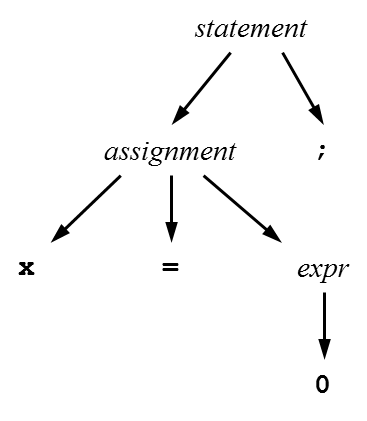
\includegraphics[width=\textwidth]{images/kapitel4/parseTreeGraph.png}
            \caption{Parse-Tree}
            \label{fig:bsp_disp_l}
        \end{subfigure}
        \begin{subfigure}[b]{0.30\textwidth}
            \centering
            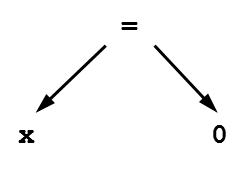
\includegraphics[width=\textwidth]{images/kapitel4/astGraph.png}
            \caption{AST}
            \label{fig:bsp_disp_r}
        \end{subfigure}
        \caption{Parse-Tree und AST der Anweisung \texttt{x = 0;}. Nachgezeichnet aus \cite{book:parrLang}.}.
	    \label{fig:Beispiel_Disparitätsbild}
\end{figure}

Der große Vorteil des AST gegenüber dem Parse-Tree ist die Unabhängigkeit von der Syntax der Sprache. Das bedeutet, dass der AST und auch  nachfolgende Verarbeitungsschritte, die auf dem AST operieren, sich nicht ändern, wenn eine Umbenennung einer Regel in der Sprache vorgenommen wird. Außerdem kann der AST schneller als der Parse-Tree durchlaufen werden, weil die Anzahl der Knoten niedriger ist. Allerdings kann der abstrakte Syntax-Baum nicht vollautomatisch aus dem Parse-Tree generiert werden, sondern nur mithilfe von Regeln, die der Kenntnis der Sprach-Semantik bedürfen und diese widerspiegeln.

%\subsection{Verwendung in dieser Arbeit}\label{ssct:4.2.1:verwendung}\todo{weg?}


\section{Implementierung und verwendete Datenstrukturen}\label{ssct:4.3:implementierung}
Die im Abschnitt \ref{sct:4.2:datenstrukturen} beschriebenen Datenstrukturen kommen - so oder in ähnlicher Form - im Rahmen dieser Abschlussarbeit vor. Ihre Implementierung und Verwendung werden in den folgenden Abschnitten detailliert beschrieben. Abbildung \ref{fig:komponenten} soll einen Überblick über die einzelnen Komponenten und ihr Zusammenspiel geben:

\begin{figure}[H]
\centering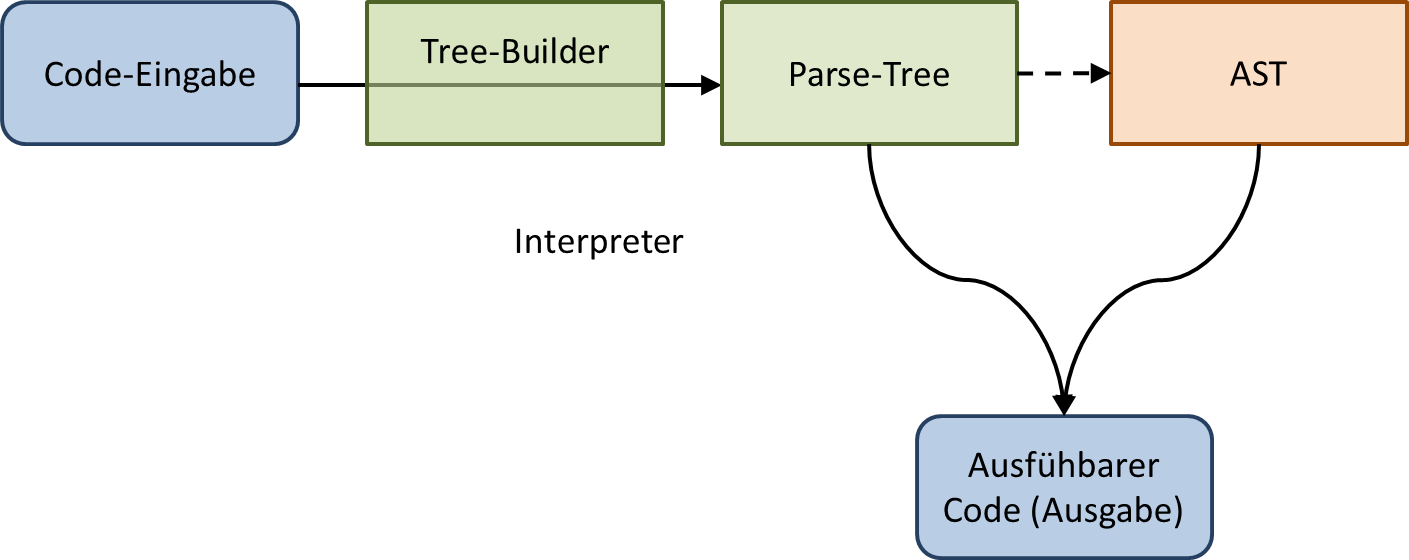
\includegraphics[width=.8\textwidth]{images/kapitel4/komponenten.png}
\caption{Komponenten der internen DSL}
\label{fig:komponenten}
\end{figure}

Die von Abschnitt \ref{ssct:4.3.1:grammatik} bis\todo{Ende} beschriebenen Implementierungen sind das Ergebnis dieser Abschlussarbeit. Abschnitt\todo{Referenz} beschreibt alternativ mögliche Implementierungen.\\
Alle nachfolgend beschriebenen Codebeispiele der Implementierung beziehen sich auf eine DSL für arithmetische Ausdrücke, genannt \textquotedblleft Expression\textquotedblright. Mit ihr lassen sich Rechnungen in den vier Grundrechenarten (\texttt{plus()}, \texttt{minus()}, \texttt{times()}, \texttt{divided}). Das erste Element eines Ausdrucks wird mit der Methode \texttt{expr()} gefasst, um eine Infix-Notation zu ermöglichen.

\subsection{Definition einer Grammatik durch Interfaces}\label{ssct:4.3.1:grammatik}
Der erste Schritt bei der Implementierung einer Sprache ist das Festlegen der Grammatik. Dies soll, wie in \ref{sct:2.3:ziel} beschrieben, nur durch Interfaces geschehen. Dabei soll es, wie in Abschnitt \ref{ssct:4.1.3:scoping} beschrieben, möglich sein, bestimmte Aufrufreihenfolgen festzulegen.\todo{restliche Beschreibung}

\begin{lstlisting}[caption={Grammatik der Expression-DSL, spezifiziert in EBNF},label=lst:grammar]
Expression ::= expr '(' ([0-9]+ | Expression) ')'
               (
                    plus '(' ([0-9]+ | Expression) ')'
                  | minus '(' ([0-9]+ | Expression) ')'
                  | times '(' ([0-9]+ | Expression) ')'
                  | divided '(' ([0-9]+ | Expression) ')'
                )*
\end{lstlisting}

\begin{figure}[H]
\centering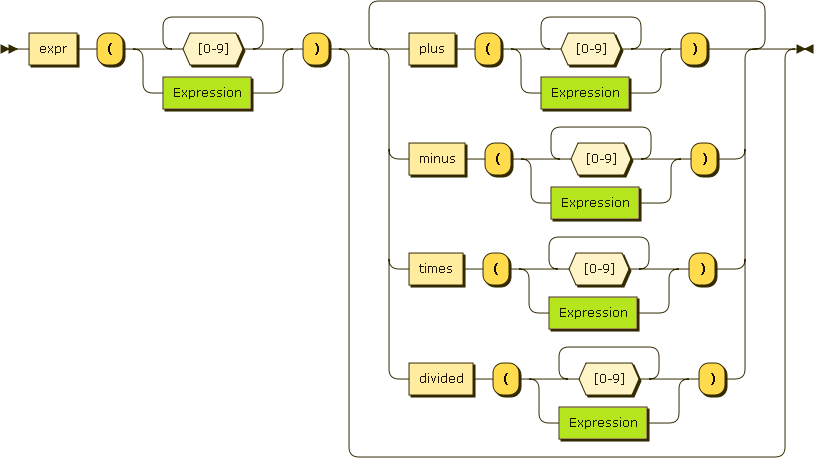
\includegraphics[width=.8\textwidth]{images/kapitel4/expressionRailroad.png}
\caption{Syntax-Diagramm der DSL}
\label{fig:railroad}
\end{figure}

Beispiel-Code

\subsection{TreeBuilder und Scopes}\label{ssct:4.3.2:treebuilder}
Damit die Methoden der durch die Interfaces definierten Grammatik aufgerufen werden können, müssen die Interfaces implementiert werden. Mithilfe von Object Scoping (siehe Abschnitt \ref{ssct:4.1.3:scoping}) wird die gewünschte Aufrufreihenfolge der Methoden festgelegt. Dazu implementiert eine Klasse \texttt{C} jeweils die Methoden eines Interfaces \texttt{I}, inklusive der Methoden derjenigen Interfaces, die \texttt{I} erweitert. Der Inhalt der Methoden dient allein dem Aufbau der Parse-Tree-Struktur (siehe auch: Abschnitt \ref{ssct:4.3.3:parsetree}) und hat keinen semantischen Inhalt. Jede der genannten Klassen - im Folgenden auch speziell Scope-Klassen genannt - hat einen privaten Konstruktor. Dadurch wird verhindert, dass unkontrolliert ein Objekt dieser Klasse instantiiert wird, wodurch die Aufrufreihenfolge verletzt werden könnte.\\
Der Zugriff auf diese Klassen und deren Methoden erfolgt über eine Builder-Klasse, in die alle Scope-Klassen als innere Klassen eingebettet werden. Diese Klasse hält eine private Instanz jeder Scope-Klasse, welche in ihrem Konstruktor erstellt wird. Jede Methode gibt entsprechend der festgelegten Aufrufreihenfolge das Scope-Objekt zurück, welches die nächste erlaubte(n) Methode(n) enthält. Auch der Konstruktor der äußeren Klasse ist privat, da eine Instanz dieser Klasse für einen User keinen Nutzen hat - alle Felder und inneren Klassen sind privat.\todo{Pattern?} Stattdessen erfolgt der Zugriff über eine statische Methode (auch Einstiegsfunktion genannt; im Beispiel: \texttt{begin()}), welche gleichzeitig den Beginn eines jeden Ausdrucks der DSL markiert. Sie ruft den Konstruktor der äußeren Builder-Klasse sowie den derjenigen inneren Klasse mit der ersten Methode auf. Sie gibt das zuletzt erstellte Objekt zurück. Danach kann die erste Methode der DSL aufgerufen werden, usw. Codeausschnitt \ref{lst:treebuilder1} zeigt beispielhaft den Code für eine Builder-Klasse.

\begin{lstlisting}[caption={Code für eine Builder-Klasse mit inneren Scope-Klassen},label=lst:treebuilder1]
public final class TreeBuilder {
	private final IntermediateScope intermediateScope;
	
	// privater Konstruktor
	private ExprDSLTreeBuilder() {
		this.intermediateScope = this.new IntermediateScope();
	}
	
	// Einstiegs-Funktion
	public static StartScope begin() {
		return new ExprDSLTreeBuilder().new StartScope();
	}
	
	public final class StartScope implements Start {

		private StartScope() {
		}

		@Override
		public IntermediateScope expr(final double value) {
			// Code	
		}
	}
	
	public final class IntermediateScope implements Intermediate {
		// ...
	}
}
\end{lstlisting}

Von der Scope-Klasse, welche die erste(n) Methode(n) eines Ausdrucks der DSL enthält, wird kein Objekt in der äußeren Klasse benötigt, da bereits die Einstiegsfunktion das entsprechende Objekt zurückgibt.



\subsection{Parse-Tree}\label{ssct:4.3.3:parsetree}


Danach:
AST erwähnen
nochmal erklären, warum Aufteilung in Grammatik, TreeBuilder, ParseTree (und AST) Vorteile mit sich bringt.
